\chapter{Monocular Depth Estimation}
\label{ch:mde}
\red{todo}
\section{Introduction to Monocular Depth Estimation}
Depth perception is the ability to determine the distance between a sensor and
the surfaces in its surroundings. It is a crucial component of robotic
navigation, mapping, and manipulation, as it allows
robots to perceive the 3D structure of their environment.
Depth perception can be performed with active sensors such as
LiDAR, ultrasonic rangefinders~\cite{Moravec_Sonar}, and
time-of-flight cameras~\cite{ToF}, or through stereo
vision~\cite{stereo}, which estimates depth by triangulating the disparity
between matched pixels in two calibrated cameras.


Monocular depth estimation (MDE), seeks to recover a depth map
from a single RGB image and no additional hardware. In this sense, the goal of MDE is most similar
to that of an RGB-D camera, which uses an infrared projector to cast a structured grid of laser dots
onto the scene and infers per-pixel depth from how that pattern is distorted by scene geometry~\cite{rgbd}; MDE
aims to recover the same dense, per-pixel depth map of an RGB image without
any active infrared projection. 


Our work leverages transformer-based machine learning models to predict 
depth of each pixel in an RGB image. MDE models are gaining more and more development
and have become more and more reliable~\cite{DPT,zoedepth, DepthAnythingV2} in the task of predicting depth.
Monocular depth estimation is particularly attractive for embedded and resource-constrained
robotic platforms, such as the cyclops rover, because it removes the need for a
dedicated depth sensor, stereo camera rig, or LiDAR unit, all of which add cost, weight,
and power draw.

The use of a camera for depth perception make the constraint
to the robot's environment: That it operate
in a well lit area


Let $I \in \mathbb{R}^{H \times W \times 3}$ denote an RGB image of height $H$ and width $W$,
and let $Z \in \mathbb{R}^{H \times W}$ denote the corresponding metric depth map. An entry $z(u,v)$ 
is the distance (in meters) along the camera's primary axis of the scene point captured by the image
at pixel $(u,v)$. Figure~\ref{fig:depth-definition} is a visual representation of this definition.
In the visualization, all points on the wall that is displayed in the captured image would have the
same metric depth. \red{consider having a 3d visualizaiton instead to capture real life}

\begin{figure}[htbp]
  \centering
  % Definition of depth z(u,v) in the metric depth map Z -- 3D view.
%
% The camera sits above the floor, pitched down towards it (about 30 deg),
% and looks along its optical axis.
% A scene point P lies on the floor, below and to the side of the camera.
% The depth of P is its distance measured along the optical axis (the Z
% coordinate in the camera frame), NOT the Euclidean distance along the ray
% from the camera to P. The depth is found by projecting P orthogonally onto
% the optical axis: P lies in the plane perpendicular to the axis that
% crosses the axis at distance z(u,v); the dotted lines inside that plane
% carry P back to the foot point F on the axis.
%
% Pure vector TikZ -- solid fills and plain paths only. Do NOT introduce
% opacity, shadings or fadings here: the Makefile builds via
% latex -> dvips -> dvipdf, where those features are unreliable.
%
% Two frames are used, both with the camera centre at the origin:
%
%   World frame (forward, lateral, up): forward = horizontal, receding into
%   the page; lateral = sideways to the camera's right; up = vertical.
%   The floor is the plane up = \H.
%
%   Camera frame (axis, lateral, camera-up): the world frame pitched down by
%   \tilt degrees about the lateral axis, so the first coordinate runs along
%   the optical axis, which points down towards the floor. The camera body,
%   optical axis, constant-depth plane and depth arrow are drawn in this
%   frame. Because the camera is pitched, the constant-depth plane is tilted
%   and meets the floor along a line rather than standing upright on it.
%
% The tilt is only for illustration and need not be exact.
\begin{tikzpicture}[>=Latex, line join=round, font=\small,
    x={(1cm,0.2cm)}, y={(0.55cm,-0.4cm)}, z={(0cm,1cm)}]

  \colorlet{depthcol}{blue!70!black}
  \def\tilt{30}  % downward pitch of the camera (degrees)
  \def\D{4}      % depth of P (along the optical axis)
  \def\L{1.4}    % lateral offset of P
  \def\H{-2.5}   % floor height (P sits on the floor)
  \pgfmathsetmacro\ct{cos(\tilt)}
  \pgfmathsetmacro\st{sin(\tilt)}
  % camera-up coordinate at which the constant-depth plane meets the floor
  \pgfmathsetmacro\hP{(\H+\D*\st)/\ct}
  % screen vectors of the pitched camera frame (world x and z rotated)
  \pgfmathsetmacro\fxs{1*\ct}\pgfmathsetmacro\fys{0.2*\ct-\st}
  \pgfmathsetmacro\uxs{1*\st}\pgfmathsetmacro\uys{0.2*\st+\ct}

  % ---- floor (world frame) ---------------------------------------------
  \fill[black!5] (-1,-1.6,\H) -- (7.2,-1.6,\H) -- (7.2,3,\H) -- (-1,3,\H) -- cycle;
  \draw[black!30] (-1,-1.6,\H) -- (7.2,-1.6,\H) -- (7.2,3,\H) -- (-1,3,\H) -- cycle;
  \node[black!50,anchor=north west] at (-1,3,\H) {floor};

  % ---- camera height above the floor (world frame) ---------------------
  \draw[black!40,dotted,thick] (-0.2,0,-0.2) -- (-0.2,0,\H);

  \begin{scope}[x={(\fxs cm,\fys cm)}, y={(0.55cm,-0.4cm)}, z={(\uxs cm,\uys cm)}]
    % key points in the camera frame
    \coordinate (F)  at (\D,0,0);      % foot point of P on the optical axis
    \coordinate (P)  at (\D,\L,\hP);   % scene point on the floor
    \coordinate (Fl) at (\D,0,\hP);    % where the depth plane meets the floor below F

    % ---- plane of constant depth through P (perpendicular to the axis) -
    \fill[black!12] (\D,-1,\hP) -- (\D,2.4,\hP) -- (\D,2.4,1.4) -- (\D,-1,1.4) -- cycle;
    \draw[black!55] (\D,-1,\hP) -- (\D,2.4,\hP) -- (\D,2.4,1.4) -- (\D,-1,1.4) -- cycle;
    \node[black!70,anchor=west,align=left,xshift=8pt] at (\D,2.4,0.4)
      {plane of\\constant depth};
  \end{scope}

  % ---- floor footprint of the camera, up to the depth plane (world) ----
  \draw[black!40,dotted,thick] (-0.2,0,\H) -- (Fl);

  \begin{scope}[x={(\fxs cm,\fys cm)}, y={(0.55cm,-0.4cm)}, z={(\uxs cm,\uys cm)}]
    % ---- camera (small box, lens facing along the optical axis) --------
    \fill[black!75] (-0.5,-0.3,-0.22) -- (-0.5,0.3,-0.22) -- (-0.5,0.3,0.22) -- (-0.5,-0.3,0.22) -- cycle;
    \fill[black!40] (-0.5,-0.3,0.22) -- (0,-0.3,0.22) -- (0,0.3,0.22) -- (-0.5,0.3,0.22) -- cycle;
    \fill[black!60] (-0.5,0.3,-0.22) -- (0,0.3,-0.22) -- (0,0.3,0.22) -- (-0.5,0.3,0.22) -- cycle;
    \node[anchor=east] at (-0.5,-0.3,0) {camera};

    % ---- optical axis in front of the depth plane ----------------------
    \draw[black!45,dashed] (0,0,0) -- (F)
      node[pos=0.5,sloped,anchor=south,yshift=-1pt,font=\footnotesize,
           text=black!55] {optical axis};

    % ---- projection of P onto the optical axis (inside the depth plane)
    \draw[black!75,dotted,thick] (P) -- (\D,\L,0) -- (F);
    \draw[black!75,dotted,thick] (P) -- (Fl) -- (F);

    % right-angle marker where the optical axis meets the depth plane
    \draw[black!65] (\D-0.35,0,0) -- (\D-0.35,0.35,0) -- (\D,0.35,0);

    % foot point on the optical axis
    \fill[black] (F) circle (1.6pt);

    % ---- Euclidean distance: the ray from the camera to P --------------
    \draw[black!75] (0,0,0) -- (P)
      node[pos=0.4,sloped,anchor=north,yshift=-1pt,font=\footnotesize,
           fill=black!5,inner sep=1pt] {Euclidean distance};

    % ---- depth z(u,v): measured along the optical axis -----------------
    \draw[|<->|,depthcol,line width=1pt] (0,0,0.6) -- (\D,0,0.6)
      node[midway,sloped,anchor=south,yshift=1pt] {depth $z(u,v)$};
  \end{scope}

  % ---- the scene point -------------------------------------------------
  \fill[black] (P) circle (2pt);
  \node[anchor=north,align=center,yshift=-3pt] at (P)
    {scene point $P$\\captured by pixel $(u,v)$};

\end{tikzpicture}

  \caption[Definition of depth in a depth map]{Definition of depth in a depth map, shown from
    above. The scene point $P$ is imaged at pixel $(u,v)$. Its depth $z(u,v)$ is the distance from
    the camera measured along the optical axis not the Euclidean distance from the camera to $P$.}
  \label{fig:depth-definition}
\end{figure}



The goal of this thesis is to develop the function $f$ described in Eq~\ref{eq:mde-map}.
Here, $\hat{Z}$ is an estimate of the true depth map $Z$, and each entry $\hat{z}(u,v)$
approximates the true depth $z(u,v)$ at pixel $(u,v)$. The function $f$ maps a single
RGB image $I$ to this estimated depth map $\hat{Z}$.
\begin{equation}
  f : \mathbb{R}^{H \times W \times 3} \rightarrow \mathbb{R}^{H \times W},
  \qquad \hat{Z} = f(I),
  \label{eq:mde-map}
\end{equation}



\section{Neural Network Architecture in Monocular Depth Estimation}
\label{sec:vit-mde}
This section provides background on the vision transformer (ViT) architecture
that state-of-the-art monocular depth estimation models employ, and motivates our
selection of Depth Anything V2 (DAv2)~\cite{DepthAnythingV2} as the depth
estimator deployed in this work. We use DAv2 as a pretrained model
without modification or fine-tuning of the underlying architecture.


\subsection{Transformers for Dense Prediction}
Early learned MDE model~\cite{MiDaS,Eigen}, used convolutional
neural network (CNN) encoder--decoder architectures, in which a convolutional backbone extracts
image features and a decoder upsamples them into a dense depth map. The Vision Transformer
(ViT)~\cite{ViT} later adapted the transformer architecture, originally developed for natural
language processing~\cite{Transformer}, to images by treating an image as a sequence of
fixed-size patches. Ranftl et al.\ replaced the convolutional encoder of MiDaS with a ViT in the
Dense Prediction Transformer (DPT), improving zero-shot depth estimation accuracy by up to $28\%$
in relative performance over a state-of-the-art fully convolutional network~\cite{DPT}.
ViT-based encoders have since become the foundation of most state-of-the-art MDE models,
including Depth Anything V2~\cite{DepthAnythingV2}, which pairs a DINOv2 ViT encoder with a
DPT decoder.

The advantage of the ViT stems from a difference in \emph{inductive bias}, the assumptions an
architecture builds in about the structure of its input. A convolution applies a small kernel to
each local neighborhood, so a CNN assumes that nearby pixels matter most and builds global context
only indirectly, by stacking layers and downsampling until its \emph{receptive field} (the region
of the input influencing a feature) covers the scene. Through self-attention, a ViT instead lets
every patch attend to every other patch, giving global context from the first layer~\cite{ViT}.
This matters for MDE because depth cues are rarely local: judging the distance to an obstacle
depends on where it meets the ground plane, the perspective lines converging toward the horizon,
and its size relative to other objects, all of which may be spread across the image.

The CNN's path to global context also carries a cost. As Ranftl et al.\ note, progressive
downsampling loses feature resolution and granularity in the deeper stages, and this detail is
difficult to recover in the decoder, which is a poor fit for dense, per-pixel tasks such as
MDE~\cite{DPT}. A ViT instead maintains a constant feature resolution throughout the encoder, so
global context is available without sacrificing spatial detail at successive stages~\cite{DPT}.




\subsection{Depth Anything V2}
\label{sec:DAV2}
Depth Anything V2~\cite{DepthAnythingV2} is the depth estimation model deployed on the Cyclops
rover. Architecturally, it is a direct instance of the encoder--decoder design described above: a
DINOv2~\cite{DINOv2} ViT encoder followed by a DPT~\cite{DPT} decoder. The input image is resized to
$518 \times 518$ pixels and divided into $14 \times 14$ patches, giving a $37 \times 37$ grid of
patch tokens that the encoder processes with self-attention. Rather than using only the final
encoder layer, DAv2 takes features from four intermediate layers of the encoder. The DPT decoder
\emph{reassembles} each set of tokens back into an image-like feature map at a different
resolution, \emph{fuses} these maps from coarse to fine, and a small convolutional head upsamples
the result into a dense relative depth map $\hat{D}$ at the input resolution.
A full treatment of the encoder and decoder is beyond the scope of this
thesis; we refer the reader to Oquab et al.~\cite{DINOv2} for DINOv2 and
Ranftl et al.~\cite{DPT} for the DPT decoder.
Figure~\ref{fig:dav2-architecture} summarizes this pipeline. In this work, the network is used
exactly as released: its weights are frozen and no layer is modified or fine-tuned.

\begin{figure}[htbp]
  \centering
  % Depth Anything V2 architecture: DINOv2 ViT encoder + DPT decoder.
%
% Shown for the ViT-S encoder deployed on the Cyclops rover (12 transformer
% layers, features tapped after layers 3, 6, 9 and 12). The whole network is
% used frozen, exactly as released.
%
% Pure vector TikZ -- solid fills and plain paths only. Do NOT introduce
% opacity, shadings or fadings here: the Makefile builds via
% latex -> dvips -> dvipdf, where those features are unreliable.
%
% Layout: top row = input, patches, encoder blocks (left to right).
%         middle row = DPT reassemble blocks, one under each encoder block.
%         bottom row = DPT fusion blocks (coarse -> fine, right to left),
%                      then the head and the output depth map.
\begin{tikzpicture}[>=Latex, line join=round, font=\small]

  \colorlet{enccol}{blue!12}
  \colorlet{deccol}{orange!15}
  \tikzset{
    blk/.style={draw=black!70, rounded corners=2pt, align=center,
                font=\scriptsize, inner xsep=1pt, minimum width=1.6cm},
    flow/.style={->, thick, black!70},
  }

  % ---- input image ----------------------------------------------------
  \fill[black!8] (0,3) rectangle (1.5,4.5);
  \fill[black!25] (0,3) -- (1.5,3) -- (1.5,3.55) -- (0,3.55) -- cycle; % floor
  \fill[black!45] (0.9,3.55) rectangle (1.25,4.05);                     % obstacle
  \draw[black!70] (0,3) rectangle (1.5,4.5);
  \node[anchor=south, align=center, font=\scriptsize] at (0.75,4.55)
    {$I$\\$518 \times 518$};

  % ---- patch grid -----------------------------------------------------
  \fill[black!8] (2,3) rectangle (3.5,4.5);
  \foreach \k in {1,2,3} {
    \draw[black!50] (2+0.375*\k,3) -- (2+0.375*\k,4.5);
    \draw[black!50] (2,3+0.375*\k) -- (3.5,3+0.375*\k);
  }
  \draw[black!70] (2,3) rectangle (3.5,4.5);
  \node[anchor=south, align=center, font=\scriptsize] at (2.75,4.55)
    {$14 \times 14$\\patches};
  \draw[flow] (1.5,3.75) -- (2,3.75);

  % ---- encoder blocks -------------------------------------------------
  \foreach \i/\lab in {1/{Layers\\1--3}, 2/{Layers\\4--6},
                       3/{Layers\\7--9}, 4/{Layers\\10--12}} {
    \pgfmathsetmacro{\x}{4.1+2.0*(\i-1)}
    \node[blk, fill=enccol, minimum height=1.1cm]
      (E\i) at (\x+0.8,3.75) {\lab};
  }
  \draw[flow] (3.5,3.75) -- (E1.west);
  \foreach \i/\j in {1/2, 2/3, 3/4} \draw[flow] (E\i.east) -- (E\j.west);

  \draw[black!55, dashed, rounded corners=4pt] (3.9,3.0) rectangle (11.9,4.95);
  \node[anchor=south east, font=\scriptsize\itshape, black!70] at (11.9,4.95)
    {DINOv2 ViT-S encoder (frozen)};

  % ---- reassemble blocks ----------------------------------------------
  \foreach \i/\s in {1/{1/4}, 2/{1/8}, 3/{1/16}, 4/{1/32}} {
    \node[blk, fill=deccol, minimum height=0.7cm]
      (R\i) at (E\i |- 0,1.95) {Reassemble\\[-1pt]$\times\,\s$};
    \draw[flow] (E\i.south) -- (R\i.north);
  }

  % ---- fusion blocks --------------------------------------------------
  \foreach \i in {1,2,3,4} {
    \node[blk, fill=deccol, minimum height=0.7cm]
      (F\i) at (E\i |- 0,0.55) {Fusion};
    \draw[flow] (R\i.south) -- (F\i.north);
  }
  \foreach \i/\j in {4/3, 3/2, 2/1} \draw[flow] (F\i.west) -- (F\j.east);

  % ---- head -----------------------------------------------------------
  \node[blk, fill=deccol, minimum width=1.5cm, minimum height=0.7cm]
    (H) at (2.75,0.55) {Head};
  \draw[flow] (F1.west) -- (H.east);

  \draw[black!55, dashed, rounded corners=4pt] (1.85,0.0) rectangle (11.9,2.55);
  \node[anchor=north east, font=\scriptsize\itshape, black!70] at (11.9,0.0)
    {DPT decoder (frozen)};

  % ---- output relative depth map --------------------------------------
  % Banded fill suggests near (bright) to far (dark) without shadings.
  \fill[black!15] (0,-0.2) rectangle (1.5,0.25);
  \fill[black!40] (0,0.25) rectangle (1.5,0.7);
  \fill[black!65] (0,0.7)  rectangle (1.5,1.3);
  \fill[black!10] (0.9,0.25) rectangle (1.25,0.75);  % near obstacle = bright
  \draw[black!70] (0,-0.2) rectangle (1.5,1.3);
  \draw[flow] (H.west) -- (1.5,0.55);
  \node[anchor=north, align=center, font=\scriptsize] at (0.75,-0.25)
    {$\hat{d}$\\relative depth\\(disparity)};

\end{tikzpicture}

  \caption[Depth Anything V2 architecture]{Depth Anything V2 architecture, shown for the ViT-S
    encoder deployed on the Cyclops rover. The image is split into $14 \times 14$ patches and
    processed by a DINOv2 ViT encoder. Features from four intermediate layers are reassembled
    into feature maps at $\tfrac{1}{4}$ to $\tfrac{1}{32}$ of the input resolution, fused from
    coarse to fine by the DPT decoder, and upsampled by the head into a dense relative depth map
    $\hat{D}$. All weights are used frozen, as released.}
  \label{fig:dav2-architecture}
\end{figure}

DAv2 is trained in two stages, each of which gives the model a property useful to the Cyclops
rover~\cite{DepthAnythingV2}. First, a teacher model is trained on roughly $595$K synthetic
images rendered from 3D scenes. Because rendered depth is exact at every pixel, including at
object boundaries where real depth sensors and stereo matching produce blurred or missing
values, the model learns to predict sharp depth discontinuities at obstacle edges, which become
sharp edges in the range scan derived in Section~\ref{sec:mde-to-range}. Second, the teacher
labels roughly $62$ million unlabeled real images, and the released models are trained on these
pseudo-labels. Exposure to this large and varied set of real scenes is what allows the model to
generalize zero-shot to our indoor environment, so it can be deployed without fine-tuning.

We use Depth Anything V2 (DAv2)~\cite{DepthAnythingV2} as the depth estimator. It is a recent
model that generalizes well zero-shot, so it can be deployed on the rover without fine-tuning,
and it is more than $10\times$ faster than recent diffusion-based estimators built on Stable
Diffusion~\cite{DepthAnythingV2}. DAv2 is released in several sizes. On standard benchmarks such as
NYU-D~\cite{NYUD}, the smallest variant is only slightly less accurate than the largest, despite
having $13\times$ fewer parameters~\cite{DepthAnythingV2}.

The Cyclops rover therefore runs DAv2-Small, the variant with the ViT-S encoder
(Figure~\ref{fig:dav2-architecture}), at $24.8$M parameters. It is also the only variant released
under the permissive Apache-2.0 license; the Base and Large models are restricted to
non-commercial use under CC-BY-NC-4.0~\cite{dav2github}. 

Even at this size, DAv2-Small runs too slowly on the rover's onboard Raspberry Pi to support
real-time navigation. Depth inference is therefore offloaded to a laptop: the rover streams each
camera frame to the laptop, which runs DAv2-Small and returns the resulting depth map.
The measured inference latency on the
laptop is reported in Chapter~\ref{ch:results}.


\section{Calibrating Metric Depth}
\label{sec:depth-calibration}

\subsection{Relative versus Metric Depth}
\label{sec:relative-depth}

Most off-the-shelf MDE models do not output meters. They output relative depth: a dense,
unitless map that is correct in ordering rather than in measurement. Metric depth, by contrast,
gives the absolute distance of each scene point from the camera in physical units (e.g.,
$50$~cm). A relative depth map can say that one pixel is nearer than another, but not whether it
is $5$~cm or $80$~cm away. That distinction matters to a motion planner deciding whether there is
clearance to pass between two objects, or to a gripper that must reach one accurately.

Models such as MiDaS and Depth Anything predict relative depth in the form of
\emph{disparity}, which, as in stereo vision, is inversely related to depth: higher values
indicate closer points~\cite{MiDaS}. We denote the predicted disparity at pixel $(u,v)$ by
$\hat{d}(u,v)$ and the corresponding metric depth by $z(u,v)$.

The main reason these models cannot output metric depth is geometric, not a deficiency that
better training could remove. As Figure~\ref{fig:scale-ambiguity} shows, an object of size $s$ at
distance $z$ and an object of size $2s$ at distance $2z$ produce identical images, so no model can
distinguish them. Absolute scale cannot be recovered from a single image alone; it requires
additional information, such as a known object size, a known camera mounting height, or a second
calibrated view. Our approach uses the known mounting height of the camera and calibrated points
on the ground plane (Section~\ref{sec:metric-scale}).

\begin{figure}[htbp]
  \centering
  % Scale ambiguity in monocular depth estimation.
%
% An object of size s at distance z and an object of size 2s at distance 2z
% subtend exactly the same visual angle, and therefore produce exactly the
% same image. Used in section 3.1.2 to motivate relative depth output.
%
% Pure vector TikZ -- solid fills and plain paths only. Do NOT introduce
% opacity, shadings or fadings here: the Makefile builds via
% latex -> dvips -> dvipdf, where those features are unreliable.
%
% Geometry: the object-subtending rays have slope 0.18 and the field-of-view
% rays slope 0.35. The near box's front face sits at x = 3.2 (half-height
% 0.576) and the far box's at x = 6.4 (half-height 1.152) -- exactly twice
% the size at exactly twice the distance.
\begin{tikzpicture}[>=Latex, line join=round, font=\small]

  % Shared fill for both objects (and their image), so they read as one
  % object. A solid xcolor mix, not opacity -- see note above.
  \colorlet{objfill}{blue!30}

  % ---- camera ---------------------------------------------------------
  \fill[black!70] (-0.45,-0.30) rectangle (0,0.30);
  \fill[black!70] (0,0) -- (0.35,0.45) -- (0.35,-0.45) -- cycle;
  \node[anchor=north] at (0,-0.55) {camera};

  % ---- field of view --------------------------------------------------
  \draw[black!45,dashed] (0,0) -- (7.6,2.66)
    node[black!55,sloped,pos=1,anchor=south east] {field of view};
  \draw[black!45,dashed] (0,0) -- (7.6,-2.66);

  % ---- rays subtending both objects -----------------------------------
  \draw[black!75] (0,0) -- (7.5,1.35);
  \draw[black!75] (0,0) -- (7.5,-1.35);

  % ---- hypothesis A: small object, near -------------------------------
  \fill[objfill]   (3.2,-0.576) rectangle (3.6,0.576);
  \draw[black!75]  (3.2,-0.576) rectangle (3.6,0.576);
  \node[anchor=south] at (3.4,0.70) {size $s$};

  % ---- hypothesis B: twice the size, twice as far ----------------------
  \fill[objfill]   (6.4,-1.152) rectangle (7.2,1.152);
  \draw[black!75]  (6.4,-1.152) rectangle (7.2,1.152);
  \node[anchor=south] at (6.8,1.28) {size $2s$};

  \node[anchor=center] at (5.0,0) {\emph{or}};

  % ---- distance measures ----------------------------------------------
  \draw[black!35,dotted] (0,-0.55)   -- (0,-3.95);
  \draw[black!35,dotted] (3.2,-0.62) -- (3.2,-2.35);
  \draw[black!35,dotted] (6.4,-1.20) -- (6.4,-3.05);
  \draw[|<->|,black!65] (0,-2.25) -- (3.2,-2.25)
        node[midway,fill=white,inner sep=1.5pt] {$z$};
  \draw[|<->|,black!65] (0,-2.95) -- (6.4,-2.95)
        node[midway,fill=white,inner sep=1.5pt] {$2z$};

  % ---- the image -------------------------------------------------------
  \draw[->,black!60,line width=0.9pt] (8.15,0) -- (8.95,0);

  \draw[black!75,fill=black!3] (9.2,-1.6) rectangle (12.2,1.6);
  \fill[objfill]  (10.1,-0.82) rectangle (11.3,0.82);
  \draw[black!75] (10.1,-0.82) rectangle (11.3,0.82);
  \node[anchor=north,align=center] at (10.7,-1.75)
        {the image $I$ produced\\by \emph{either} object};

\end{tikzpicture}

  \caption[Scale ambiguity in monocular depth estimation]{Scale ambiguity in monocular depth
    estimation. An object of size $s$ at distance $z$ and an object of size $2s$ at distance $2z$
    both produce the identical image $I$.}
  \label{fig:scale-ambiguity}
\end{figure}

Several recent models do predict metric depth directly~\cite{DepthAnythingV2,MoGe}, but they
work around the ambiguity by learning scale cues from their training data, such as typical object
sizes and camera viewpoints. The metric variants of DAv2, for example, are fine-tuned on the
synthetic indoor dataset Hypersim~\cite{hypersim} and on Virtual KITTI 2~\cite{virtualkitti2},
which uses a car-mounted camera~\cite{DepthAnythingV2}. A camera mounted close to the floor on a
small rover departs from both, and in our preliminary trials the metric DAv2 models were
noticeably less accurate on the Cyclops rover (errors of about $20$~cm, for obstacles $40$~cm away) and added
roughly $100$~ms of inference latency. We therefore use a relative depth model and recover metric
scale from the rover's own geometry. A formal comparison is left to future work.
\subsection{Affine-Invariant Disparity Output}
\label{sec:alignment}
To convert relative depth into metric depth, we need the exact relationship between
$\hat{d}(u,v)$ and $z(u,v)$, which is set by how the model is trained. Zero-shot MDE models
require tens of millions of training images~\cite{ViT,DepthAnythingV2}, so they are trained on a
mixture of sources: LiDAR scans, indoor RGB-D captures, web stereo photographs,
structure-from-motion reconstructions, and frames from 3D films~\cite{MiDaS,DPT}. These sources do
not share a common scale or shift. Stereo photographs and films, for instance, provide disparity
without the focal length and baseline needed to convert it to meters. Ranftl et
al.~\cite{MiDaS} resolved this by solving, for each training image, the scale $a$ and shift $b$
that best fit the prediction to the ground truth, and penalizing only the error that remains.
Depth Anything V2 is trained the same way~\cite{DepthAnythingV2}. Because $a$ and $b$ are fitted
away during training, the network never learns their values, and its output is correct only up to
an unknown affine transform in disparity space:
\begin{equation}
  \frac{1}{\hat{z}(u,v)} \;=\; a\,\hat{d}(u,v) + b
  \label{eq:affine-disparity}
\end{equation}

This has two consequences for our work. First, recovering metric depth reduces to estimating two
scalars, since the network already supplies the per-pixel structure of the scene. Second, because
$a$ and $b$ were fitted separately for every training image, nothing keeps them constant from one
frame to the next, so a one-time calibration is not enough. The Cyclops rover therefore
re-estimates $a$ and $b$ on every frame from ground-plane pixels whose metric depth is known from
the camera's mounting geometry (Section~\ref{sec:metric-scale}).


\subsection{Recovering Metric Scale}
\label{sec:metric-scale}

To estimate $a$ and $b$ in Equation~\eqref{eq:affine-disparity}, we exploit the mounting
geometry of the camera. The Cyclops rover drives on a flat floor, and its camera is rigidly
mounted to the front of the chassis (Figure~\ref{fig:cyclops-rover}), so the height and tilt of
the camera relative to the ground never change. Consequently, a pixel that images the floor
always images the same point on the floor relative to the camera, and the metric depth at that
pixel stays constant from frame to frame. Such pixels provide a fixed set of reference depths
against which every new prediction can be aligned.

This method of recovering metric scale give our second constraint to the robot's 
environmeny: that
it operates on a ground plane and anything above that ground plane is an obstacle

We select $N = 96$ of these pixels, which we call \emph{ground points}. Let
$(u_k, v_k)$ denote the image location of the $k$-th ground point and $z^{\mathrm{g}}_k$ its known
metric depth, for $k = 1, \dots, N$.

Figure~\ref{fig:ground-points} shows the checkerboard target used to obtain the ground points.
The checkerboard is laid flat on the floor in front of the rover, and each of its inner corners
serves as one ground point; the figure annotates every corner with its depth $z^{\mathrm{g}}_k$ (meters).
Because the size of the checkerboard squares is known, the 3D position of each corner in the
checkerboard's own coordinate frame is also known. Given these 3D positions, their detected pixel
locations, and the camera intrinsics, OpenCV's \texttt{solvePnP} function~\cite{opencv_library} estimates the rotation
and translation of the checkerboard relative to the camera by solving the Perspective-n-Point
problem~\cite{solvepnp}. Applying this transformation yields the coordinates of every corner in the
camera frame. We keep only the $z$ coordinate, since depth along the optical axis is the quantity
that MDE predicts.

\begin{figure}[htbp]
  \centering
  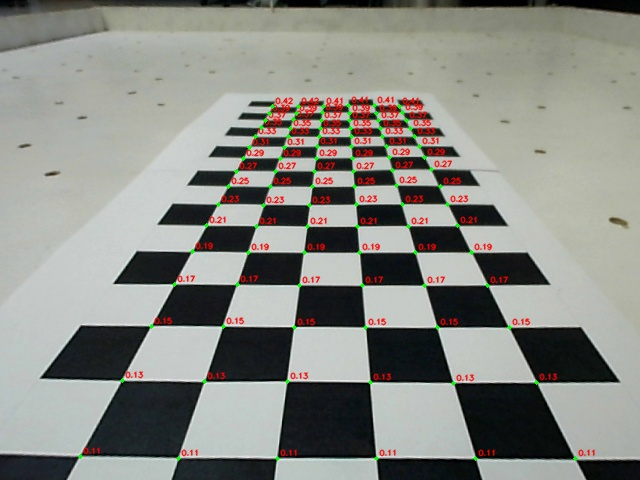
\includegraphics[width=0.8\textwidth]{figures/annotated_depth_ref13.jpg}
  \caption{Checkerboard target on the floor in front of the Cyclops rover. Each inner corner is a
    ground point, annotated with its metric depth $z^{\mathrm{g}}_k$ (meters).}
  \label{fig:ground-points}
\end{figure}

\red{Do I have to justify }
With the ground points fixed, the alignment parameters are recalculated on every frame. For a new image,
let $\hat{d}^{\mathrm{g}}_k = \hat{d}(u_k, v_k)$ denote the model's relative disparity at the $k$-th ground
point. By Equation~\eqref{eq:affine-disparity}, the known depths should satisfy
$1/z^{\mathrm{g}}_k \approx a\,\hat{d}^{\mathrm{g}}_k + b$. Equation~\eqref{eq:ridge-fit} depicts the ridge
regression objective minimized to find $a$ and $b$, where $\lambda > 0$ is a regularization weight
that discourages large values of the scale.
\begin{equation}
  (a^{*}, b^{*}) \;=\; \arg\min_{a,\,b} \;\sum_{k=1}^{N}
    \left( a\,\hat{d}^{\mathrm{g}}_k + b - \frac{1}{z^{\mathrm{g}}_k} \right)^{2} + \lambda\,a^{2}
  \label{eq:ridge-fit}
\end{equation}
The fitted $a^{*}$ and $b^{*}$ are then substituted into Equation~\eqref{eq:affine-disparity} to
convert the relative disparity $\hat{d}(u,v)$ at every pixel into inverse metric depth $1/\hat{z}(u,v)$.


We over sampled the points but it was also good for obstacle and to confirm that
the output was truly linear.

During devlopment we only needed to do two rows and did a relative depth
that is smaller than the closer row (obstacle )





\section{Monocular Depth to Range Finder}
diagram of image to mde to laptop etc
that we foudn too slow on embedded hardware with no GPU thus moving to laptop
\label{sec:mde-to-range}


\subsection{Back-Projection to 3D}

 A scene
point $(X, Y, Z)$ expressed in the camera frame projects to
\begin{equation}
  u = f_x \frac{X}{z} + c_x,
  \qquad
  v = f_y \frac{Y}{z} + c_y,
  \label{eq:projection}
\end{equation}
and, given a depth $z$ at pixel $(u,v)$, the corresponding scene point is recovered by
back-projection:
\begin{equation}
  X = \frac{(u - c_x)\, z}{f_x},
  \qquad
  Y = \frac{(v - c_y)\, z}{f_y},
  \qquad
  Z = z .
  \label{eq:backprojection}
\end{equation}
Equation~\eqref{eq:backprojection} is the mechanism by which Section~\ref{sec:mde-to-range}
converts a depth map into the geometry of a range scan.

red{Figure sth hows a sample of the point cloud}

\subsection{Ground-Plane and Ceiling Deletion}

\subsection{Reduction to a 1D Angular Range Scan}
\todo{The step that makes a camera behave like a range finder. The bearing of image column $u$ is
$\theta(u) = \arctan\!\big((u - c_x)/f_x\big)$; partition the horizontal field of view into $K$
angular bins matching the beam layout the measurement model of Chapter~\ref{ch:localization}
expects, and take the minimum surviving obstacle range within each bin. Define the maximum usable
range and the encoding of invalid or no-return beams.}

\subsection{Noise Characterization}
\todo{Characterize the error distribution of the resulting ranges as a function of true distance
and bearing, including the heavy tail produced by depth-boundary bleed at object silhouettes.
This distribution is the input to the beam model $p(z_t \mid x_t, m)$ in
Chapter~\ref{ch:localization}.}

\subsection{Entire MDE diagram}

%%% Local Variables: ***
%%% mode: latex ***
%%% TeX-master: "thesis.tex" ***
%%% End: ***
